%!TEX root = thesis.tex

%
%==========================================================================================
%
\chapter{Anomalous and Suspicious Behavior Detection}
\label{chap:detection}

This chapter discusses how to approach anomalous and suspicious behavior detection. It first formalizes the problem and shows how to optimally perform detection. It then discusses why optimal detection is not always possible, proves the lower error bound and discusses heuristics approaches. Finally, it describes how to design multi-view detectors and combine their evaluations. 

%
%==========================================================================================
%
\section{Detection Objectives}

Our focus is detection of deviant behavior patterns that might represent a security risk, health problem, or any other abnormal behavior contingency. Such patterns occur  infrequently; however, when they do occur, their consequences can be quite dramatic, and  often negatively. Typical examples include credit card fraud detection, cyber intrusions, industrial damage, etc. 

\index{feature extraction}
More formally, we define behavior pattern as follows:
\begin{definition}
\index{behavior pattern}
	\emph{Behavior pattern} $\bsig$ is a vector of features extracted from behavior trace $\mathbf{b}=\{(a, s)_t | 1 \leq t \leq T\}$.
\end{definition}
\noindent
The definition implies that a behavior pattern can be constructed from a behavior trace by an arbitrary function. The main idea is to introduce a set of features that effectively encodes the behavior trace, such as the spatio-activity matrix introduced in Chapter~\ref{chap:signatures}.


% is related to the lack of complete pos false alarms
%For example, 
\index{behavior!deviant behavior}
We use term \emph{deviant behavior} to refer to behavior that is either suspicious or anomalous and cast the deviant behavior detection problem in a statistical framework, which builds upon \cite{Helman1993} intrusion detection framework. This will help introduce rigorous notions, which are required later in the thesis, and allow future work to evolve toward broader objectives.

At time step $t$, we observe a behavior pattern $\bsig_t$, generated by a hidden stochastic process $H$. Now suppose that $H$ is a mixture of two auxiliary stochastic processes, namely the normal process $N$ and the suspicious process $S$, that correspond to a legitimate and a deviant behavior of an agent, respectively. The random variable $y_t=0$ if $\bsig_t$ is generated by $N$ and $y_t=1$ if $\bsig_t$ is generated by $S$. 
%Since an anomalous agent always emits an anomalous behavior pattern (and a legitimate agent a legitimate pattern), $y$ for a specific agent does not change over time. 
In reality, there can be many subprocesses contributing to both $N$ and $S$; that is, many legitimate agents with different behavior patterns or an agent with many legitimate and deviant behavior profiles. However, here we assume only a single $N$ and a single $S$ that capture all the variability. 

To this point, we have assumed that an observer is able to observe perfectly whether a behavior pattern is generated by $S$ or $N$. In practice, however, it may appear that a legitimate agent emits deviant behavior patterns (or vice-versa). An observer might be limited for various reasons, such as an inability to detect characteristic features, and noisy activity recognition models. Therefore, we relax this assumption as follows: a behavior pattern $\bsig_t$ is observed as generated by $N$ with the probability 
\begin{equation}
	n(\bsig_t) = \Prob\{H(t)=\bsig_t|y_t=0\},
\end{equation}
and as generated by $S$ with the probability 
\begin{equation}
	s(\bsig_t) = \Prob\{H(t)=\bsig_t|y_t=1\}.%= 1 - n(\bsig_t).
\end{equation}
Given the preceding assumption, that is, \emph{a priori} probability $\lambda$ that a behavior pattern is legitimate, the mixture distribution of a pattern $\bsig_t$ is
\begin{equation}
  \Prob\{H(t)=\bsig_t\} = \lambda n(\bsig_t) + (1-\lambda) s(\bsig_t).
\end{equation}
\noindent
Note that in most applications, $\lambda$ is close to 1, since deviant behavior patterns are rare, necessitating the application of modeling techniques such as those described in the next section.

We illustrate via a simple example the above-mentioned definitions and concepts. Suppose the behavior pattern consists of only two features, \emph{activity} and \emph{landmark}, and that the possible values for \emph{activity} are $\mathbb{A}=\{standing, lying\}$, while the possible values for \emph{landmark} are $\mathbb{S}=\{kitchen, bedroom\}$. Hence, the spatio-activity space can be presented by the set $\{\tuple{kitchen, standing}, \tuple{kitchen, lying}, \tuple{bedroom, standing}, \tuple{bedroom, lying}\}$ of ordered pairs.
Assume the following probability distribution on spatio-activity space for $1 \leq t \leq T$:
\begin{eqnarray*}
\Prob\{H(t)=\tuple{kitchen, standing}|y_t=0\} 	= n(\tuple{kitchen, standing}) &=& 0.950, \\
\Prob\{H(t)=\tuple{kitchen, lying}|y_t=0\}  	= n(\tuple{kitchen, lying}) &=& 0.020, \\
\Prob\{H(t)=\tuple{bedroom, standing}|y_t=0\}  = n(\tuple{bedroom, standing}) &=& 0.250, \\
\Prob\{H(t)=\tuple{bedroom, lying}|y_t=0\} 	= n(\tuple{bedroom, lying}) &=& 0.850,\\
\Prob\{H(t)=\tuple{kitchen, standing}|y_t=1\}  = s(\tuple{kitchen, standing}) &=& 0.020, \\
\Prob\{H(t)=\tuple{kitchen, lying}|y_t=1\}  	= s(\tuple{kitchen, lying}) &=& 0.900, \\
\Prob\{H(t)=\tuple{bedroom, standing}|y_t=1\}  = s(\tuple{bedroom, standing}) &=& 0.050, \\
\Prob\{H(t)=\tuple{bedroom, lying}|y_t=1\} 	= s(\tuple{bedroom, lying}) &=& 0.050.
\end{eqnarray*}

Then, if, for example, $\lambda=0.9$, the mixture probability is:
\begin{eqnarray*}
\Prob\{H(t)=\tuple{kitchen, standing}\} 	&=& 0.857, \\
\Prob\{H(t)=\tuple{kitchen, lying}\} 		&=& 0.108, \\
\Prob\{H(t)=\tuple{bedroom, standing}\} 	&=& 0.230, \\
\Prob\{H(t)=\tuple{bedroom, lying}\} 		&=& 0.770.
\end{eqnarray*}

The objective of behavior detection is to identify those patterns that are likely to be deviant activities, that is, patterns $\bsig$ for which
\begin{equation}
		\Prob\{y_t=1|H(t)=\bsig_t\} > \tau,
\label{eq:detect}
\end{equation}
is above some threshold $\tau$ or is large relative to the probability for other traces.

According to Bayes theorem and our definitions
\begin{equation}
\begin{aligned}
\Prob\{y_t=1|H(t)=\bsig_t\} = \\
& = \frac{(1-\lambda)\Prob\{H(t)=\bsig_t|y_t=1\}}{(1-\lambda)\Prob\{H(t)=\bsig_t|y_t=1\} + \lambda \Prob\{H(t)=\bsig_t|y_t=0\}}\\
& = \frac{(1-\lambda)s(\bsig)}{(1-\lambda)s(\bsig) + \lambda n(\bsig)}\\
& = \frac{(1-\lambda)r(\bsig)}{(1-\lambda)r(\bsig) + \lambda}\\
& = \frac{r(\bsig)}{r(\bsig) + \lambda/(1-\lambda)},
\end{aligned}
\label{eq:detect-bayes}
\end{equation}
\noindent
where $r(\bsig)=s(\bsig)/n(\bsig)$ if $n(\bsig) > 0$, and $r(\bsig)=\infty$ if $n(\bsig)=0$. We derive from Equation~(\ref{eq:detect}) and Equation~(\ref{eq:detect-bayes}) that a behavior pattern is deviant iff:
\begin{equation}
		r(\bsig) > \frac{\lambda \tau}{(1-\lambda)(1-\tau)}.
\label{eq:detect-condition}
\end{equation}

Assuming the probabilities in the previous example, we can compute
\begin{eqnarray*}
r(\tuple{kitchen, standing}) 	&=& 0.021, \\
r(\tuple{kitchen, lying}) 		&=& 0.450, \\
r(\tuple{bedroom, standing}) 	&=& 0.200, \\
r(\tuple{bedroom, lying})		&=& 0.059.
\end{eqnarray*}

However, in practice, some or all of the probabilities for the above calculations are unknown. We have no direct knowledge of the \emph{a priori} probability $\lambda$ and distribution of processes $N$ and $S$. Our primary concern is hence to develop models that estimate the likelihood of ratio $r(\bsig)$ and, therefore, distributions $s(\bsig)$ and $n(\bsig)$. 

% \begin{definition}
% 	\emph{Behavior evaluation} is a function
% 	$$
% 	f: \mathbb{R}^{||\mathcal{B}||} \rightarrow \mathbb{R}
% 	$$
% 	that assigns a real value to a behavior pattern as a degree of suspiciousness or anomalousness. It is expressed as a probability of 
% \end{definition}
% \noindent



%
%==========================================================================================
%
\section{Detection Performance}
\index{detector}
\index{detection performance}
First, we define \emph{detector} as a behavior signature ranking mechanism. The larger the value provided by the detector, the more deviation is attributed to the signature.
\begin{definition}
\index{detector!graded detector}
	\emph{Graded detector} $D_g$ is a function from behavior signature space $\tilde{\mathbb{B}}$ to non-negative real set:
	$$
	D_g: \tilde{\mathbb{B}} \rightarrow \mathbb{R}_0^+.
	$$
\end{definition}
\begin{definition}
\index{detector!binary detector}
	\emph{Binary detector} $D_g$ is a function from behavior signature space $\tilde{\mathbb{B}}$ to binary set:
	$$
	D_b: \tilde{\mathbb{B}} \rightarrow \{0,1\}.
	$$
\end{definition}
\noindent
For any graded detector $D_g$, we can associate a set of binary detectors $D_{b, \tau}$ satisfying
\begin{equation}
		D_{b, \tau} = \begin{cases}
		   1; & D_g \geq \tau \\
		   0; & \text{else }
		  \end{cases}.
\label{eq:freq-n}
\end{equation}
\noindent
For example, we could define a graded detector as $D_g(\bsig)=r(\bsig)$. Similarly, we could define a binary detector $D_b(\bsig)=1$ if $r(\bsig) \geq \lambda/(1-\lambda)$ and $D_b(\bsig)=0$ otherwise.

In general, legitimate process $N$ and deviant process $S$ may overlap, which means that for some signatures $\bsig$, both $n(\bsig)$ and $s(\bsig)$ are non-zero. Therefore, a detector (graded or binary) can map two signatures to the same value, even if one was generated by $N$ and the other by $S$. Consequently, some error is unavoidable.

\index{detection performance!true positive}
\index{detection performance!false positive}
\index{detection performance!true negative}
\index{detection performance!false negative}
There are four possible outcomes as shown in Table~\ref{tab:outcome}. The first column contains possible signatures (deviant or legitimate), while the first line contains detector outcomes. 
\begin{table}[!ht]
\centering
\caption{Detection outcomes.}
\renewcommand{\arraystretch}{1.2}
\begin{tabular}{ccc}
\toprule
							& Detector: legitimate					& Detector: deviant					\\
	\hline
	Deviant signature		& miss (false negative)					& hit (true positive)			\\
	Legitimate signature	& correct rejection	(true negative)		& false alarm (false positive)	\\
\toprule
\end{tabular}
\label{tab:outcome}
\end{table}
\index{detection performance!type II error}
\index{detection performance!type I error}
There are two types of error: type I error or false positive, which can be thought of as \emph{convicting a legitimate agent}; and type II error or false negative; that is, \emph{letting a suspicious agent go free}. A perfect detector would have $0\%$ false negatives and $0\%$ false positives; that is, it would correctly identify all deviant and legitimate signatures. However, theoretically any detector will possess a minimum error bound if the distributions $N$ and $S$ overlap.

Figure~\ref{fig:error} illustrates an example of overlapping distributions $N$ and $S$ \citep{Duda2000}. The red and blue shaded areas in the tail of distributions $N$ and $S$ represent type I and type II errors, respectively. An arbitrarily chosen decision point $\tau*$ represents the binary detector's decision boundary; that is, regions $D_b(\bsig)=0$ and $D_b(\bsig)=1$. The marked triangular area represents \emph{reducible error}, which can be eliminated if the decision boundary is moved to $\tau_{opt}$, the optimal decision boundary, which gives the lowest error probability.

\begin{figure}[!ht]
\centering
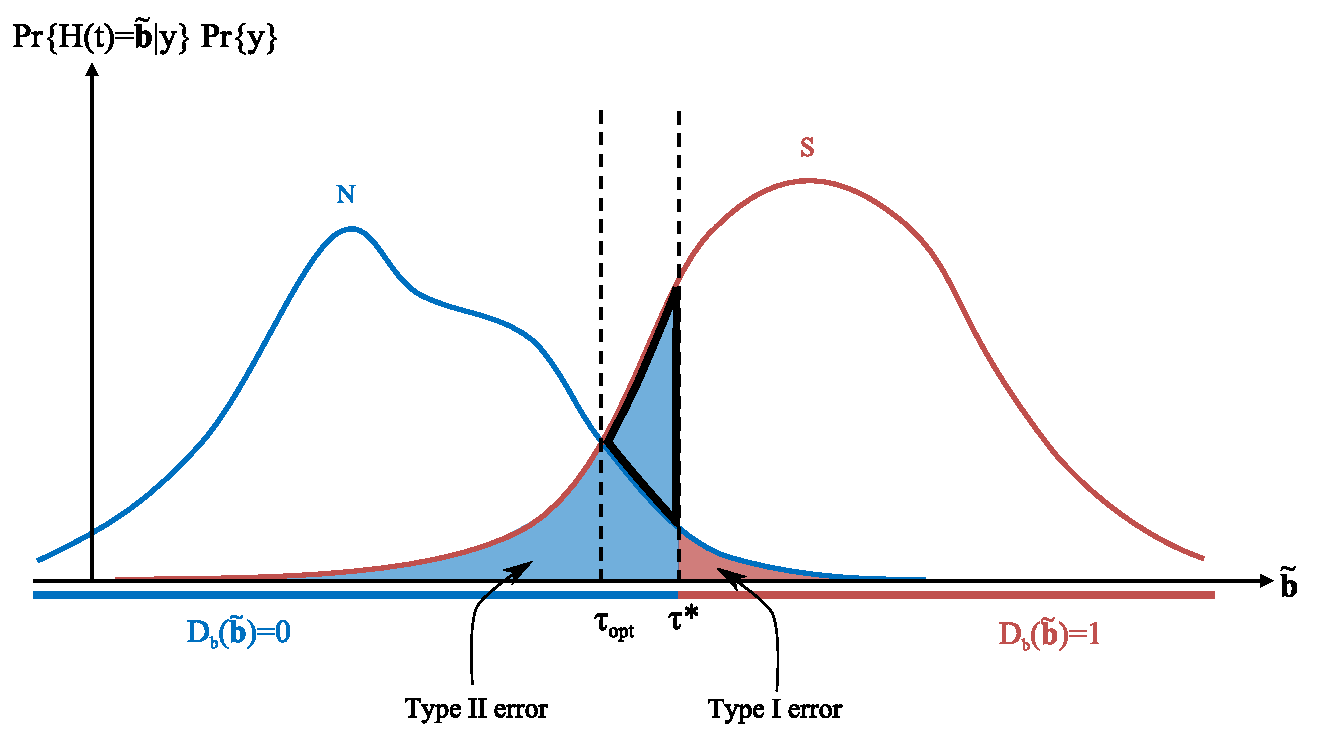
\includegraphics[width=0.9\textwidth]{chap_DET/error}
\caption{Overlapping distributions $N$ and $S$.}
\label{fig:error}
\end{figure}


\begin{theorem}
For any binary detector $D_b$, the symmetric error is bounded below by
$$
\sum_{t=1}^T \min{(s(\bsig_t) (1-\lambda), n(\bsig_t) \lambda)}.
$$
\end{theorem}
\begin{proof}
The error probability consists of two terms; that is, type I and type II errors as shown in Equation~(\ref{eq:det-error}).
\begin{equation}
\begin{aligned}
		\Prob\{error\} 
		&= \sum_{\substack{t=1 \\ D_b(\bsig)=0}}^T s(\bsig_t) \Prob\{y=1\} + \sum_{\substack{t=1 \\ D_b(\bsig)=1}}^T n(\bsig_t) \Prob\{y=0\} \\
		&= \sum_{\substack{t=1 \\ D_b(\bsig)=0}}^T s(\bsig_t) (1-\lambda) + \sum_{\substack{t=1 \\ D_b(\bsig)=1}}^T n(\bsig_t) \lambda
\end{aligned}
\label{eq:det-error}
\end{equation}
\noindent
As follows from Equation~(\ref{eq:det-error}), it is advantageous to classify a behavior signature $\bsig$ as legitimate if $s(\bsig_t) (1-\lambda) < n(\bsig_t) \lambda$ so that the smaller quantity will contribute to the error sum; the other way around follows analogously. Consequently, the lower error bound as defined in the theorem's statement is achieved.
\end{proof}

Frequently, the type I and type II errors are not considered of equal importance; hence, we can weight them with two constants $\alpha, \beta \in [0,1]$ s.t. $\alpha+\beta=1$. The error probability then follows from Equation~(\ref{eq:det-error-nonsym}). 
\begin{equation}
\begin{aligned}
		\Prob\{error\} 
		&= \alpha \sum_{\substack{t=1 \\ D_b(\bsig)=0}}^T s(\bsig_t) (1-\lambda) + \beta \sum_{\substack{t=1 \\ D_b(\bsig)=1}}^T n(\bsig_t) \lambda
\end{aligned}
\label{eq:det-error-nonsym}
\end{equation}

%A reasonable performance measure is defined as a wighted harmonic mean of 


%
%------------------------------------------------------------------------------------------
%

\subsection{Performance Measures}
\index{detection performance!sensitivity}
\index{detection performance!specificity}
\index{detection performance!precision}
\index{detection performance!F-measure}
Optimality conditions assume that detection is performed with the benefit of perfect information. In practice, knowledge of distributions is not readily available and the detectors are evaluated on a behavior-signature database. 
The common performance measures are:
\begin{itemize}
	\item \emph{sensitivity}, also \emph{true positive rate} or \emph{recall} -- the proportion of deviant signatures, which are correctly identified as such
		\begin{equation}
				\text{sensitivity} = \frac{\text{TP}}{\text{TP}+\text{FN}},% = 1 - \textit{type I error},
		\label{eq:sensitivity}
		\end{equation}
	\item \emph{specificity}, or \emph{true negative rate} -- the proportion of correctly identified legitimate signatures
		\begin{equation}
				\text{specificity} = \frac{\text{TN}}{\text{TN}+\text{FP}},% = 1 - \textit{type II error},
		\label{eq:specificity}
		\end{equation}
	\item \emph{precision}, or \emph{positive predictive value} -- the proportion of correctly raised alarms
		\begin{equation}
				\text{precision} = \frac{\text{TP}}{\text{TP}+\text{FP}}.
		\label{eq:precision}
		\end{equation}
\end{itemize}
In addition, sensitivity and precision, that is, the fraction of detected deviant signatures and the fraction of relevant alarms are ideally close to $100\%$ (that is, no type I and type II errors). \emph{F-measure} considers both the precision and the recall to compute the score as a weighted precision and recall average, where the score reaches its best value at 1 and worst at 0. 
\begin{equation}
	F = 2 \cdot \frac{\text{precision} \cdot \text{recall}}{\text{precision} + \text{recall}}
\label{eq:F-measure}
\end{equation}



%
%------------------------------------------------------------------------------------------
%
\subsection{False Positive Paradox}
%http://en.wikipedia.org/wiki/False_positive_paradox

\index{false positive paradox}
The false positive paradox~\citep{Rheinfurth1998} occurs when the behavior signature-database has a low deviant behavior signature share and the detector's hit rate is lower than the false positive rate. In this case, the false positive test is more probable than the true positive test.

Consider the following example:  suppose a detector $D$ has false alarm rate $0.04\%$ and false negative rate (miss) $0\%$; that is, it marks all deviant signatures.  Now suppose we have a behavior signature database $\mathcal{B}_A$ with a million signatures in which $2$ of $100$ signatures are deviant; that is, $2\%$. The detection scores are as follows:
\begin{equation*}
\begin{aligned}
\text{TP} &= 1,000,000 * 0.02 * 1.0 = 20,000 \text{ signatures (hits)},\\
\text{FP} &= 1,000,000 * 0.98 * 0.0004 = 392 \text{ signatures (false alarms)}.
\end{aligned}
\label{eq:paradox-example1}
\end{equation*}
Hence, a signature is classified as deviant with over $98\%$ confidence; that is, $precision=20,000/20,392$.

Now suppose the same detection is applied to a behavior signature database $\mathcal{B}_B$ in which $1$ of $10,000$ signatures are deviant; that is, $0.01\%$. The detector in this case scores as follows:
\begin{equation*}
\begin{aligned}
\text{TP} &= 100,000 * 0.0001 * 1.0 = 100 \text{ signatures (hits)},\\
\text{FP} &= 100,000 * 0.9999 * 0.0004 \approx 400 \text{ signatures (false alarms)}.
\end{aligned}
\label{eq:paradox-example1}
\end{equation*}
A signature is now classified as deviant with only $20\%$ confidence, since only $100$ of total $500$ signatures marked as deviant are indeed deviant. Given the results on database $\mathcal{B}_A$, it is considered paradoxical that deviant detection is mostly a false alarm in database $\mathcal{B}_B$. The probability of a deviant detection result is hence determined not only by the accuracy of the detection, but also by the distribution of the sampled behavior signatures. Hence it is crucial that historical behavior signature distribution matches the behavior signature distribution on which the detector is applied.



%
%==========================================================================================
%
\section{Detectors}
\index{detector}
\cite{Helman1993} divided detectors into: \emph{modeling approaches}, which require estimation of distributions $s(\bsig)$ and $n(\bsig)$ to directly attack the problem of deviant behavior detection, for example, neural networks~\citep{Biermann2001}, k-nearest neighbors \citep{Govindarajan2009}, na\"ive-Bayes estimators \citep{Kruegel2003}; and \emph{non-modeling approaches} that do not explicitly estimate $s(\bsig)$ or $n(\bsig)$, but use various heuristics to flag deviant behavior patterns, for example, expert rules~\citep{Esponda2004}, plan recognition~\citep{Avrahami-Zilberbrand2007}, and decision trees~\citep{Ektefa2010}.

%Approaches for estimating $r(\bsig)$ include neural networks, k-nearest neighbors, na\"ive-Bayes estimators, 

%
%==========================================================================================
%
\subsection{Frequentist Estimator}
\index{frequentist estimator}
Frequentist estimator is a basic approach that estimates distributions $n(\bsig)$ or $s(\bsig)$. The distribution $n(\bsig)$ is estimated from a historical database of behavior signatures $\mathcal{B}$:
\begin{equation}
		\bar{n}(\bsig) = \Prob\{\bsig\} = \frac{\eta(\bsig) }{|\mathcal{B}|},
\label{eq:freq-n}
\end{equation}
\noindent
where $\eta(\bsig)$ counts the number of the occurrences of the signature $\bsig$ in $\mathcal{B}$.

Two promising models for estimating distribution $s(\bsig)$ are \emph{uniform} and \emph{independence} model.
The uniform model assumes that all signatures are equally likely, regardless of the historical database:
\begin{equation}
		\bar{s}_u(\bsig) = \frac{1}{|\bsig|}.
\label{eq:freq-n}
\end{equation}
\noindent
The \emph{independence} model assumes that the features in the behavior signature $\bsig=\langle f_1, ..., f_L \rangle$ are independent, that is:
\begin{equation}
		\bar{s}_i(\bsig) = \Prob\{f_1, \dots, f_L\} = \prod_{i=1}^{L}{\Prob\{f_i\}}  = \prod_{i=1}^{L}\frac{\eta(f_i)}{|\mathcal{B}|}.
\label{eq:freq-n}
\end{equation}

The models are best illustrated by means of example. Consider a behavior signature structure from the previous example. Suppose further that the historical database consists of $100$ signatures, yielding observed frequencies of the four possible behavior signatures as shown in Table~\ref{tab:freq-example}.
\begin{table}[!ht]
\centering
\caption{Example: Observed frequencies of four possible behavior signatures.}
\renewcommand{\arraystretch}{1.2}
\begin{tabular}{ccc}
	\toprule
	Activity / Landmark		& Kitchen	& Bedroom	\\
	\hline
				Standing	& 3 		& 8			\\
				Lying		& 7 		& 82			\\
	\toprule
\end{tabular}
\label{tab:freq-example}
\end{table}

The frequentist estimator gives us, for example, $\bar{n}(\tuple{kitchen, standing})=0.030$ and $\bar{n}(\tuple{kitchen, lying})=0.070$. With the uniform model, we obtain $\bar{s}_u(\bsig)=0.25$ for any $\bsig$, which gives us ratios $\bar{r}_u(\tuple{kitchen, standing})=8.333$ and $\bar{r}_u(\tuple{kitchen, lying})=3.571$. The uniform model simply exposes signatures less likely to be generated by process $N$, without any reference to process $S$. Hence, the signature $\tuple{kitchen, standing}$ is considered as anomalous, as it is the least frequent in the historical database. 

The independence model gives us $\bar{s}_i(\tuple{kitchen, standing})=0.011$ and $\bar{s}_i(\tuple{kitchen, lying})=0.089$, leading us to ratios $\bar{r}_i(\tuple{kitchen, standing})=0.367$ and $\bar{r}_i(\tuple{kitchen, lying})=1.271$. In this case, the signature $\tuple{kitchen, lying}$ is marked as suspicious because activity \emph{lying} is something relatively unusual to be performed at landmark \emph{kitchen}.


Each of the models is clearly better than the other for certain tasks. While we believe those basic models to be reasonable starting points, we envision a framework in which several models are combined to yield the final evaluation.

%
%==========================================================================================
%
\subsection{Density Estimator}

 The estimation can be based on a distance measure to deviant and legitimate behavior signatures in the historical database $\mathcal{B}$. Suppose the historical database $\mathcal{B}$ can be split into legitimate $\mathcal{B}_n$ and deviant $\mathcal{B}_s$ signatures. The ratio $r(\bsig)$ can be then defined as a ratio between distance to the $k$-nearest legitimate and deviant signatures:
\begin{equation}
		r(\bsig) = \frac{\sum_{\bsig_i \in nn(\bsig, \mathcal{B}_s)}^k d(\bsig, \bsig_i)}{\sum_{\bsig_i \in nn(\bsig, \mathcal{B}_n)}^k d(\bsig, \bsig_i)},
\label{eq:density-r}
\end{equation}
\noindent
where $d$ is a distance measure (for example, Manhattan, Euclidean, or Mahalanobis distance) and $nn$ is a set of signatures ordered by the distance to behavior signature $\bsig$:
\begin{equation}
		nn(\bsig, \mathcal{B})=\{\bsig_1, \bsig_2, \cdots, \bsig_{|\mathcal{B}|}| d(\bsig, \bsig_i) \leq d(\bsig, \bsig_{i+1})\}.
\label{eq:density-nn}
\end{equation}

Practical applications are frequently faced with absence of one of the $\mathcal{B}_n$ or $\mathcal{B}_s$ databases. In this case, the detection is focused on one of the tasks: \emph{suspicious} or \emph{anomalous} behavior detection \citep{Avrahami-Zilberbrand2009}.

 %(\cite{Avrahami-Zilberbrand2009}), where the preceding assumption is that a set of historical behavior patterns $\mathcal{B}$ is already available.
%In other words, deviant behavior is a pattern in the data that either does not conform to the expected behavior (anomalous behavior) or matches previously defined unwanted behavior (suspicious behavior). Deviant behavior patterns are also referred to as outliers, exceptions, peculiarities, surprise, misuse, etc. 

\index{behavior!suspicious behavior}
\begin{definition}
	Consider a set of behavior patterns $\mathcal{B}_s$ that encodes negative (suspicious) behavior. A behavior pattern $\mathbf{b} \not \in \mathcal{B}_s$ is \emph{suspicious} iff
	$$
	\exists \mathbf{b}_i \in \mathcal{B}_s: d(\mathbf{b}, \mathbf{b_i}) < \epsilon.
	$$
\end{definition}
\noindent
In other words, a behavior pattern is considered suspicious if it matches at least one suspicious behavior pattern. 
Since suspicious behavior is usually rare, this approach requires an expert that specifies all the suspicious patterns. Thus, such detection systems can only discover threats that are known {\it a priori}. 
Examples include models that encode possible attacks in intrusion detection systems~\citep{Biermann2001}, trying to identify if an attack is under progress; and models with fall-dynamic templates in remote eldercare systems~\citep{Lee04daily} that are compared to observation to infer whether the situation matches one or more templates.


\index{behavior!anomalous behavior}
The other approach uses a set of behavior patterns in an inverse fashion.
\begin{definition}
	Consider a set of behavior patterns $\mathcal{B}_n$ that encode positive (normal) behavior. A behavior pattern $\mathbf{b} \not \in \mathcal{B}_n$ is \emph{anomalous} iff
	$$
	\forall \mathbf{b}_i \in \mathcal{B}_n:  d(\mathbf{b}, \mathbf{b_i}) > \epsilon'.
	$$
	%where $\Phi(\mathbf{b}, k)$ is a set of $k$ patterns $\mathbf{b}_i$ ordered by the distance to $\mathbf{b}$ ($k$-nearest patterns).
	%$$
	%\Phi(\mathbf{b}, k) = \{b_j| d(\mathbf{b}_j, \mathbf{b}) < d(\mathbf{b}_{j+1}, \mathbf{b}), 1 \leq j \leq k \leq |\mathcal{B}_p|\}.
	%$$
\end{definition}
\noindent
The set of behavior patterns is limited to covering only positive, expected behavior patterns. If a behavior pattern cannot be matched against those patterns, it is announced as anomalous. An advantage of this approach is that it requires only examples of positive behavior, which are usually abundant and attainable. This approach can thus detect unforeseen threats and contingencies. However, one potential issue is false positives caused by an incomplete legitimate behavior set; that is, a legitimate behavior pattern is marked as anomalous if it was not previously included in the set $\mathcal{B}_n$. 
%Examples of anomalous behavior detection include models of legitimate person activities... 


\index{local outlier factor, LOF}
A notable approach is Local Outlier Factor (LOF)~\citep{Breunig00lof}, an outlier-detection algorithm based on computing the local neighborhoods densities. The main idea of the LOF algorithm is to assign to each signature a degree of being an outlier. This degree is the LOF of a vector. Vectors with a high LOF have local densities smaller than their neighborhood and typically represent stronger outliers, unlike vectors belonging to uniform clusters that usually tend to have lower LOF values. 
Due to the local approach, LOF is able to identify outliers in a data set that would not be outliers in another area of the same data set. For example, a point at a small distance to a very dense cluster is an outlier, while a point within a sparse cluster might exhibit similar distances to its neighbors.
%The main advantages of the LOF algorithm are that: (i) it detects outliers with respect to local density, not global model; and (ii) it is able to detect outliers regadless of the data distribution (since it does not make any assumptions about distribution). 

%Assume that $A$ is a set of daily-behavior traces $A={B_1, B_2, ..., B_n}$. To detect an anomalous behavior trace we apply the procedure described in Algorithm~\ref{alg:LOF}. First, for each behavioral trace $B_i$ compute the spatio-activity matrix $M_i$ using Algorithm~\ref{alg:SA_matrix}, then compute the vector $p_i$ of the principal components (Equation~\ref{eq:PCA-1}-\ref{eq:PCA-4}), and add vector $p_i$ to the new dataset $A'$. Next, for each vector $p_i$ compute the $k\_dist_i$ as the distance to the $k^{th}$ nearest neighbor of $p_i$,  compute the reachability distance for each vector $p_i$ with respect to the vector $p_j$, where $d(p_i,p_j)$ is the Euclidean distance from $p_i$ to $p_j$, and compute the local reachability density $lrd_i$ of the vector $p_i$ as the inverse of the average reachability distance based on the $k$ nearest neighbors of the vector $p_i$. Finally, compute the $LOF_i$ of the vector $p_i$ as the ratio of the average local reachability density of $p_i$'s  $k$ nearest neighbors and the local reachability density of the vector $p_i$.


% \begin{algorithm}
% \caption{Anomaly detection.}
% \label{alg:LOF}
% \begin{algorithmic}
% \REQUIRE set of behavior traces $A={B_1, B_2, ..., B_n}$, number of $k$ nearest neighbors
% \ENSURE outlier degree for each behavior trace $LOF_i$
% \STATE $A' \gets \{\}$
% \FOR {$B_i \in A$}
% 	\STATE $M_i \gets sa\_matrix(B_i)$
% 	\STATE $p_i \gets PCA(M_i)$
% 	\STATE $A' \gets A' \cup p_i $
% \ENDFOR
% \FOR {$p_i \in A'$}
% 	\STATE $k\_dist_i \gets k\_distance(p_i)$
% 	\FOR{$p_j \in A', p_j \neq p_i$}
% 		\STATE $r\_dist_{i,j} \gets max(d(p_i, p_j), k\_dist_j))$
% 	\ENDFOR
% 	\STATE $lrd_i = {k \over { \sum_{p_j\in kNN(p_i)}{r\_dist_{i, j}}}}$
% 	\STATE $LOF_i \gets { {1 \over k}{{ \sum_{p_j\in kNN(p_i)}{lrd_j}}} \over lrd_i}$
% \ENDFOR
% \end{algorithmic}
% \end{algorithm}

\index{feature extraction}
The more behavior signature features, the more likely each signature is unique, and the less likely that any fixed size historical set represents a substantial mass of all signatures; that is, any density estimator becomes less reliable.

%
%==========================================================================================
%
\subsection{Machine Learning Approaches}

Detectors employ statistical models generated from historical signatures automatically or by an expert. They specify relationships between the values of features and target value. For example, a rule might state if the landmark is \emph{kitchen} and activity is \emph{lying}, then signature is \emph{suspicious}.

If no historical signature is available, an expert specifies a set of rules covering either desired (legitimate) or unwanted (deviant) behavior. Detection is performed analogously as in the previous section.

Data-driven rule generation is defined as a classification task, which constructs a model able to exploit statistical differences in a database of historical behavior signatures. Notable approaches are decision trees, SVMs, neural networks, etc.



%
%==========================================================================================
%
\section{Combining Multiple Detectors}
\label{sec:combine}

As indicated in several studies, it is often advantageous to combine decisions of several experts to reach the final conclusion~\citep{Woods1996, Gams2011principle, Vilalta02}. A single detector might be weak in certain aspect; that is, unable to reliably detect or evaluate specific behaviors. 
For example, consider the ambient assisted living domain. An anomalous event, such as fall, must be detected within seconds, while gradual degradation of gait resulting in limping might require months to be manifested. A detector specialized for anomalous events on the \textit{seconds} scale would be unable to detect such degradation; analogously, a detector  operating on \textit{months} scale would simply filter out events such as falls. The combination of both would address both behaviors to provide anomalous events detection.

The main idea is to construct several local views; that is, detectors trained on a subset of complete feature space such as modalities differences, time scales,  contextual information, and detection method approaches, into the final evaluation.


There are several possible strategies for performing the final evaluation: first, all detectors are considered equally important/reliable; second, accept the decision delivered by the most reliable expert ignoring majority consensus; third, weight detectors by their importance/past perfomance/reliability. A promising direction is to utilize expert knowledge to encode the last approach in a form of a Bayesian network as a set of random variables and their conditional dependencies via a directed, acyclic graph. For example, a Bayesian network could represent the probabilistic relationships between the behavior in question and detectors. Given detectors' evaluations, the network can be used to compute the probabilities that the behavior deviates.


\section{Summary and Discussion}
This chapter helped to understand the anomalous and suspicious behavior detection problem, and why it is difficult to solve. The chapter gave the first clear problem definition and established a theoretical framework for anomalous and suspicious behavior detection from agent traces. We showed how to optimally perform detection, discussed why detection error is often inevitable, and proved the lower error bound. We further provided several heuristic approaches that either estimated distributions required to perform detection or directly rank the behavior signatures using machine-learning approaches.

The main assumption of this chapter was that the decision must is based on a single agent observation. In practice, however, there are often many observations available, which allows the observer to make a decision based on multiple observations. The next chapter extends the theoretical framework to address multiple observations, discusses emerged issues, and proposes an approach to evaluate multiple observations.



%that specifies releationship

%TODO: allow several local views - detectors trained on a subset of complete feature space, they can be weak

%TODO: two possible strategies: all experts are considered equally reliable/important OR accept the decision delivered by the most reliable expert ignoring majority consensus.

% Each human tends to perform activities in a specific way, be it on the micro or macro scale. However, the behavior of the persons in our system is actually monitored from three different points of view. In the first of these, denoted as the \textit{micro level}, one typically deals with behavior that changes in tenths of a second or seconds. For example, one person always carries his identity card in a wallet and puts the whole wallet near the wireless identity-card reader, while another person carries her card in a handbag and requires some time to take it out, identify herself, and put the card back. The person's movement around the access point depends on his/her habits and mental/physical state. These facts determine the persons' patterns at the micro level.

% The second viewpoint, denoted as the \textit{macro level}, describes the persons' daily routines. The activities of interest are the arrival times at access points, the movements between various access points in the access-control network, and even the connections between persons, for example, person $A$ often enters a short time after person $B$. The time scale used at the macro level can vary from seconds to months.

% The third viewpoint, denoted as the \textit{visual level}, captures the persons' visual movement at an access point using a camera. It is also focused on micro-level movements; that is, behavior that changes over a short time interval, but in addition to micro-level features, it obtains features from the visual characteristics of the person and his/her movement, for example, the person's height and the door-opening dynamics.

% Several rules additionally control the regular entry procedure, the regular working time, and the access permissions.


%\section{Time Scales}
%\section{Modalities}

%\subsection{A Bayesian Network Model}

% After the expert rules, micro, macro, visual and meta-learning have made their assessments, their results are integrated into a joint risk analysis of the current entry. It estimates the probability of the event $E = $ \textit{entry is regular} given the observations of the modules. If the estimated probability does not exceed a threshold value, an alarm is triggered. Note that an alarm can also be triggered by expert rules when there is sufficient certainty (type 1 rules).

% The reasoning in the prototype system is performed with a Bayesian network, structured as shown in Figure~\ref{fig:bayesianNetwork}. Four modules have a direct impact on the event $E$; that is, expert rules, micro learning and visual learning, and a macro meta-learning module, while the macro meta-learning module depends only on the three macro modules. The probabilities in the network are computed from the test data, using the \textit{m-estimate}  for conditional probabilities and the \textit{Laplace estimate} for a-priori probabilities. 
% \begin{figure}[h]
% \centering
% \includegraphics[bb=0 540 440 800,width=8cm]{eswa/BayesNetwork2}
% %\includegraphics[bb=30 590 360 820,width=8cm]{img/BayesNetwork.pdf}
% %\includegraphics[bb=0 540 440 800,width=8cm]{img/BayesNetwork2.pdf}
% \caption{Bayesian network used for the reasoning.}
% \label{fig:bayesianNetwork}
% \end{figure}

% The integration proceeds in three steps. Firstly, the output from each module is converted to interval the $[0, 1]$ representing the a-posterior probability $p_{M_i}$ that the entry is regular. Secondly, given the Bayesian network $N$ and the probabilities $p_{M_i}$, the estimated  probability of an event $E$ is computed from the network.
% %\begin{eqnarray}
% %P(E | M_1, M_2, \dots, M_n) = P(E) \frac{P(M_1, M_2, \dots, M_n | E)}{P(M_1, M_2, \dots, M_n)}
% %\end{eqnarray}
% %Numerator is developed with chain rule and due to the structure of the network is simplified to:
% %\begin{multline}
% %P(M_1, M_2, \dots, M_n | E) = \prod_{i=1}^{n} P(M_i | Parents(M_i)) = \\
% % = \prod_{i=1}^{n} p_{M_i} P(M_i=1|E) + (1-p_{M_i}) P(M_i=0|E)
% %\end{multline}
% %Denominator, on the other hand, is independent of the event E, thus is developed as follows:
% %\begin{multline}
% %P(M_1, M_2, \dots, M_n) = \\
% % = \sum_{e\in\{0, 1\}} P(E=e) P(M_1, M_2, \dots, M_n | E=e)  =\\
% % = \sum_{e\in\{0, 1\}} P(E=e) \prod_{i=1}^{n} (p_{M_i} P(M_i=1|E=e) + \\
% % + (1-p_{M_i}) P(M_i=0|E=e))
% %\end{multline}

% Finally, the integration module outputs the joint analysis as a probability that the entry is regular and provides an explanation. According to the threshold values, the integration module triggers \textit{alarm} or \textit{OK} and stores the results in the ontology. In high-security areas, the cost of a false alarm is negligible compared to the cost of an unrecognized intruder; therefore, the system is set to minimize the latter.

